\documentclass[12pt]{article}
\usepackage{amsmath,amsthm,amssymb}
\usepackage{mathtext}
\usepackage[T1,T2A]{fontenc}
\usepackage[utf8]{inputenc}
\usepackage[english,russian]{babel}
\usepackage{titling}
\usepackage{float}
\usepackage{graphicx}
\usepackage[section]{placeins}
%\usepackage[a4paper, total={7in, 10in}]{geometry}
\usepackage[margin=1in,footskip=0.25in]{geometry}

\graphicspath{ {./images/} }

\begin{document}

\title{Алмазная кубическая решетка в EAM-LJ потенциале}
\author{Никитюк Борис}
\date{}
\maketitle
%\newpage
%\tableofcontents
\newpage

\section{Введение}
Для описания взаимодействия в металлах и расплавах необходим учет многочастичных взаимодействий, в частности взаимодействий частиц метала с электронным газом. Одним из способов учета таких взаимодейстий является потенциал погруженного атома, разработанный Daw и Baskes [1]. Для описания взаимодействий помимо парных взаимодействий вводится функция погружения, описывающая взаимодействие атома с некой обобщенной конфигурацией системы. Baskes представил вариант такого потенциала, основанный на потенциале Леннарда-Джонса [2]. В этом проекте представлена реализация этого потенциала и изучение некоторых свойств алмазной кубической решетки в нем. 

\section{Методы и техника расчета}
\subsection{Теория}
Для однокомпонентной схемы EAM потенциал задается тремя функциями - погружения $F(\rho)$, парного взаимодействия $\phi(r)$ и плотностью электронных облаков $\rho(r)$. Потенциальная энергия в нем выражается, как 

\begin{equation}
E=\sum_{i}\left[F\left({\rho}_{i}\right)+\frac{1}{2} \sum_{j \neq i} \phi\left(r_{i j}\right)\right]
\end{equation}

В работе [2] предлагается ввести функции основываясь на потенциале Леннарда-Джонса:

\begin{subequations}
\begin{align}
& F(\rho)=\frac{A Z_{0}}{2} \rho [\ln (\bar{\rho})-1] \\
& \phi(r)=\phi_{\mathrm{LJ}}(r)-\frac{2}{Z_{0}} F(\rho(r)) \\
& \rho_{i}=\frac{1}{Z_{0}} \sum_{j \neq i} \rho\left(r_{i j}\right) \\
& \rho(r)=\exp [-\beta(r-1)]
\end{align}
\end{subequations}

Для получения сил, необходимо продифференцировать полную энергию по координате соответствующего атома (для удобства перенесем нормировочную константу $Z_0$ в функцию погружения).

\begin{equation}
\begin{aligned}
&\vec{F}_{i}=-\vec{\nabla}_{\vec{r}_{i}} E =
-\vec{\nabla}_{\vec{r}_{i}} \sum_{i} E_i =
-\vec{\nabla}_{\vec{r}_{i}} \left[F_i \left(\rho_{i} \right)+\sum_{j \neq i} F_{j}\left(\rho_{j} \right) + \sum_{j \neq i} \phi_{ij} \left(r_{ij}\right)\right]=\\
&=-\sum_{j \neq i}\left[\left.\left.\frac{\partial F_{i}(\rho)}{\partial \rho}\right|_{\rho=\rho_{i}}\frac{\partial \rho_{ji}(r)}{\partial r}\right|_{r=r_{j}}+
\left.\left.\frac{\partial F_{j}(\rho)}{\partial \rho}\right|_{\rho=\rho_{j}} \frac{\partial \rho_{ij}(r)}{\partial r}\right|_{r=r_{j}}+
\left.\frac{\partial \phi_{i j}(r)}{\partial r}\right|_{r=r_{j}}\right] \frac{\left(\vec{r}_{i}-\vec{r}_{j}\right)}{r_{i j}}= \\
&=-\sum_{j \neq i}\left[\frac{\partial F_{i}(\rho_i)}{\partial \rho_i}\frac{\partial \rho_{ji}(r_{ij})}{\partial r_{ij}}+
\frac{\partial F_{j}(\rho_j)}{\partial \rho_j}\frac{\partial \rho_{ij}(r_{ij})}{\partial r_{ij}}+
\frac{\partial \phi(r_{i j})}{\partial r_{ij}}\right] \frac{\left(\vec{r}_{i}-\vec{r}_{j}\right)}{r_{i j}}
\end{aligned}
\end{equation}

Таким образом, для расчета сил так же как и в случае обычного потенциала Леннарда-Джонса, достаточно расстояния между двумя частицами. Подставляя в выражения для силы и энергии можно получить выражения для них в явном виде:

\begin{equation}
\vec{F_{i}} = \vec{F_{\mathrm{LJ}}} + \sum_{j \neq i} \left[\frac{A\beta}{2} e^{-\beta (r_{ij}-1)} ln\left(\rho_i \rho_j\right) + A \beta^2 e^{-\beta (r_{ij}-1)} (r_{ij}-1) \right] \frac{\vec{r_{ij}}}{r_{ij}}
\end{equation}

\begin{equation}
E_{i} = E_{\mathrm{LJ}} - \frac{A}{2} e^{-\beta (r_{ij}-1)} (-\beta (r_{ij}-1) - 1) + \frac{A Z_0}{2} \rho_i (ln(\rho_i)-1)
\end{equation}

Таким образом взаимодействие частиц зависит от двух констант $A$ и $\beta$, где $A$ описывает силу взаимодействие, а $\beta$ - размеры электронных облаков, то есть длину на которой взаимодействие существенно.

\subsection{Практическая реализация}
Заметим, что при вынесении расчета плотности элетронных облаков в отдельный цикл, алгоритм рассчета сохраняет асимптотику $O(N^2)$. 

Важно так же отметить, что формулы, полученные в предыдущем параграфе из предложенных в [2], получены для $r$ выраженных в $2^{1/6} \sigma$. Поэтому при реализации кода была учтена соответствующая нормировка.

Все расчеты были произведены без обрезки потенциала. Число частиц, шаг интегрирования указан в каждом конкретном случае.

Для проверки корректности выведенных выражений и из практической реализации можно проверить сохранение полной энергии.

\begin{figure}[h]
\centering
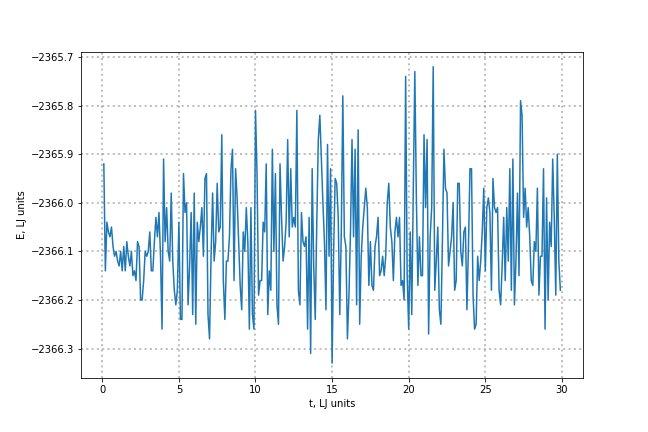
\includegraphics[width=1.0\textwidth]{energy5}
\caption{Полная энергия от времени, N=512, $\Delta t = 10^{-3}$, T=0.5}
\end{figure}
\FloatBarrier

Флуктуация энергии: $\left\langle \Delta E^2 \right\rangle /E = 5\times 10^{-5}$. Отсюда, энергия сохраняется. Большая часть расчетов в этом проекте производится при меньших температурах, где энергия флуктуирует еще меньше.

При температурах близких к 0 для этой же системы флуктуация энергии значительно падает: $\left\langle \Delta E^2 \right\rangle /E = 2\times 10^{-6}$.
 
\begin{figure}[h]
\centering
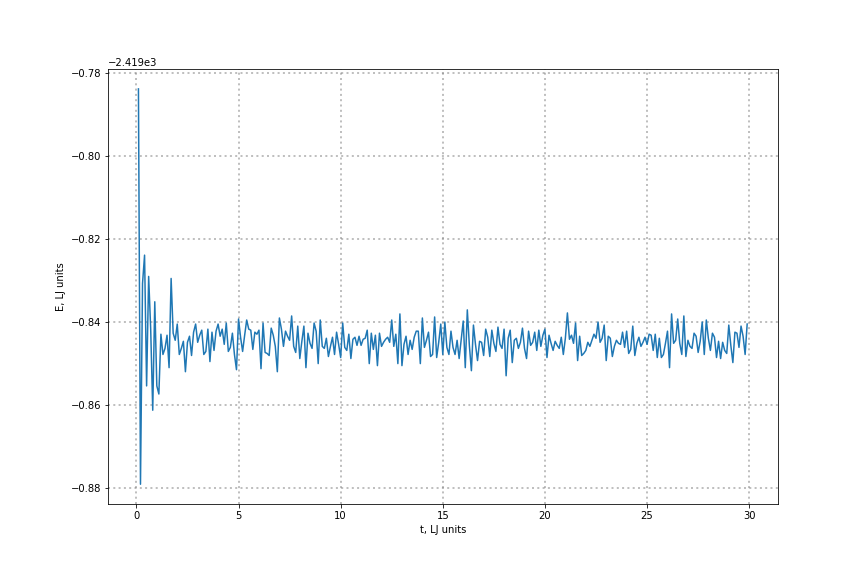
\includegraphics[width=1.0\textwidth]{energy1}
\caption{Полная энергия от времени, N=512, $\Delta t = 10^{-3}$, T=0.015}
\end{figure}
\FloatBarrier

\section{Результаты и анализ}
\subsection{Образование решеток}
Одним из преимуществ EAM потенциала является возможность получения различных типов решеток в зависимости от заданных параметров $A$ и $\beta$. Baskes в работе [2] приводит диаграмму устойчивых состояний: 
\begin{figure}[h]
\centering
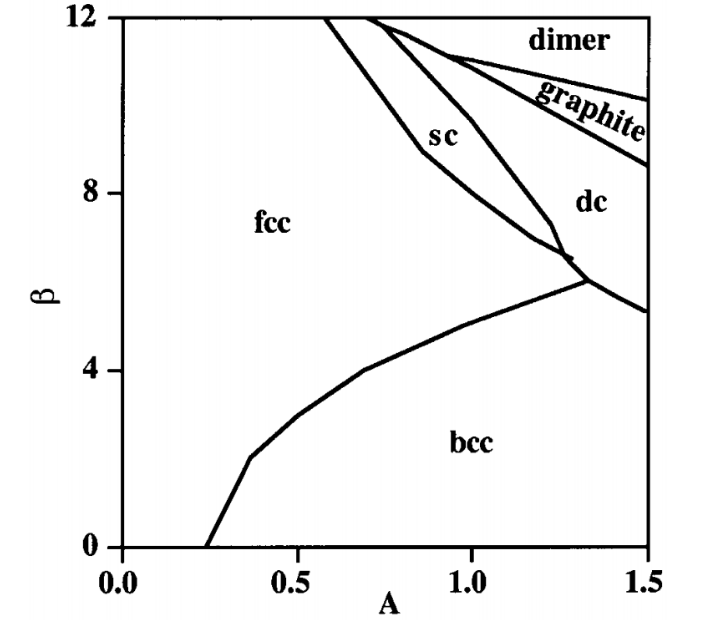
\includegraphics[width=0.5\textwidth]{phases_baskes}
\caption{Устойчивые решетки, Фазовая диаграмма системы в зависимости от параметров $A$ и $\beta$ из статьи Baskes, “Many-Body Effects in fcc Metals”.}
\end{figure}
\FloatBarrier

Мне удалось получить соответствующие решетки:
\begin{figure}[h]
\centering
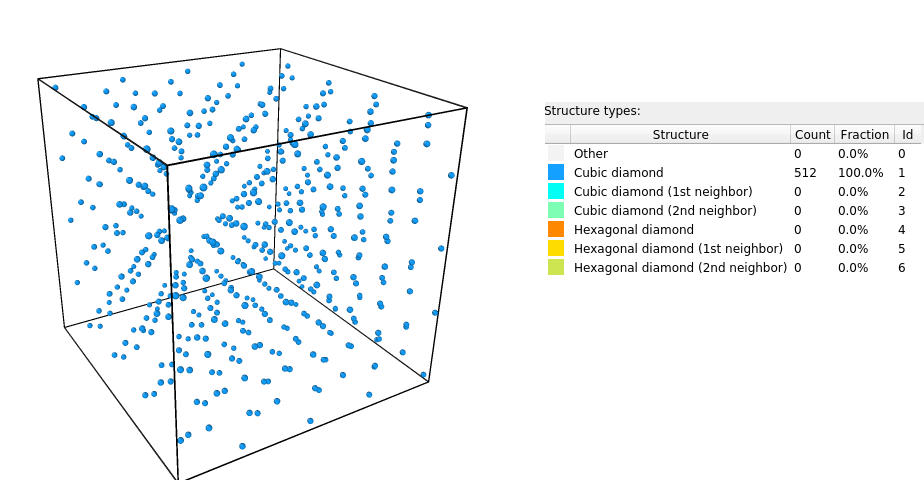
\includegraphics[width=0.81\textwidth]{dc_all}
\caption{dc-решетка. $A=1.5 \ \beta=6$}
\end{figure}
\FloatBarrier
\begin{figure}[h]
\centering
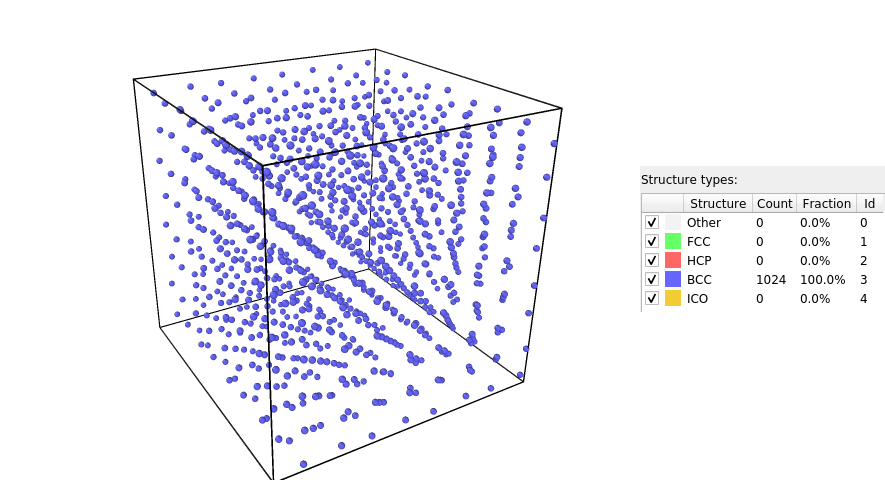
\includegraphics[width=0.9\textwidth]{bc_all}
\caption{bcc-решетка. $A=1 \ \beta=2$}
\end{figure}
\FloatBarrier
\begin{figure}[h]
\centering
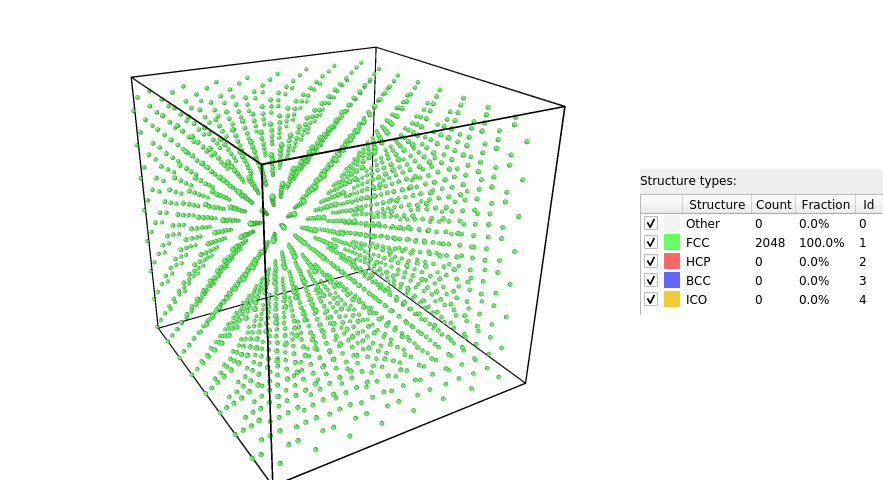
\includegraphics[width=0.9\textwidth]{fcc_all}
\caption{fcc-решетка. $A=0.5 \ \beta=6$}
\end{figure}
\FloatBarrier

Для анализа типа решетки были использованы функции "Common neighbor analysis" [3] и "Identify diamond structure" [4] OVITO.

Так же, возможен выбор значений постоянных вне графика на рисунке 3. 

\begin{figure}[h]
\centering
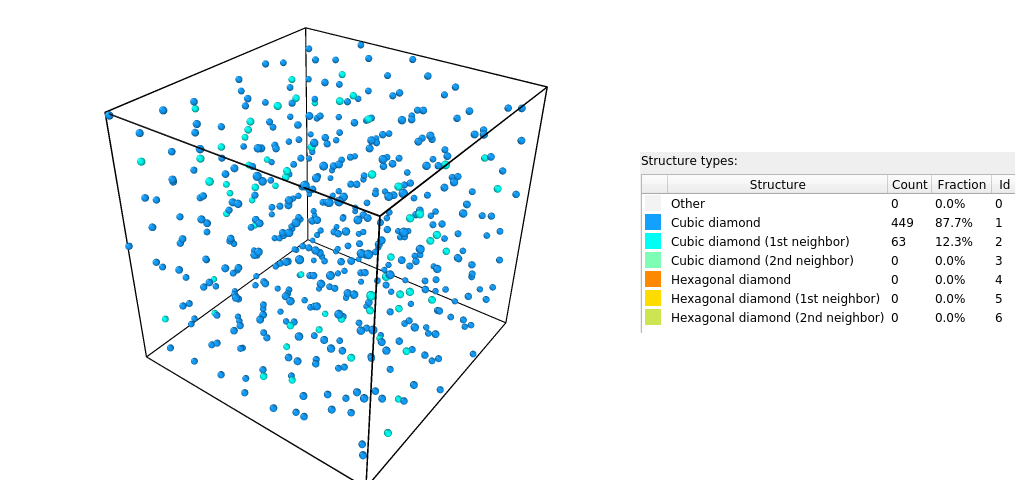
\includegraphics[width=0.8\textwidth]{bc10_all}
\caption{dc-решетка. $A=10 \ \beta=7 \ T=0.15$}
\end{figure}
\FloatBarrier

Другим способом анализа структуры является функция радиального распределения. Построим ее для алмазной кубической решетке, изучаемой в дальнейшем. Отношение координат пиков: $1.63 = \sqrt{8/3}$, что соответствует dc-решетке [2]. 

\begin{figure}[h]
\centering
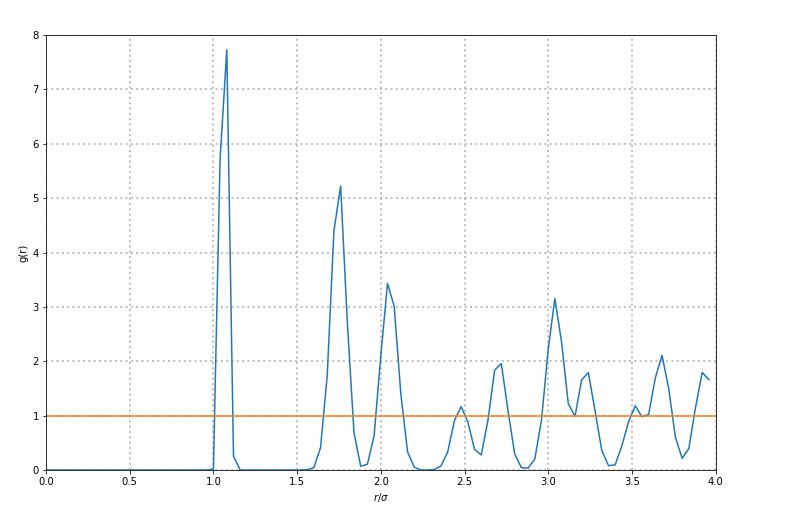
\includegraphics[width=0.80\textwidth]{radial}
\caption{RDF dc-решетки. $N=512, A=1.5, \beta=6, \rho=0.512$}
\end{figure}
\FloatBarrier

\newpage
\subsection{Температура плавления}

Baskes в работе [2] приводит зависимость температуры плавления от констант потенциала - она уменьшается с повышением обеих констант. Продолжая его на область, в которой стабильна dc-решетка, получаем, что при температурах отличных от 0, решетка должна плавиться.

\begin{figure}[h]
\centering
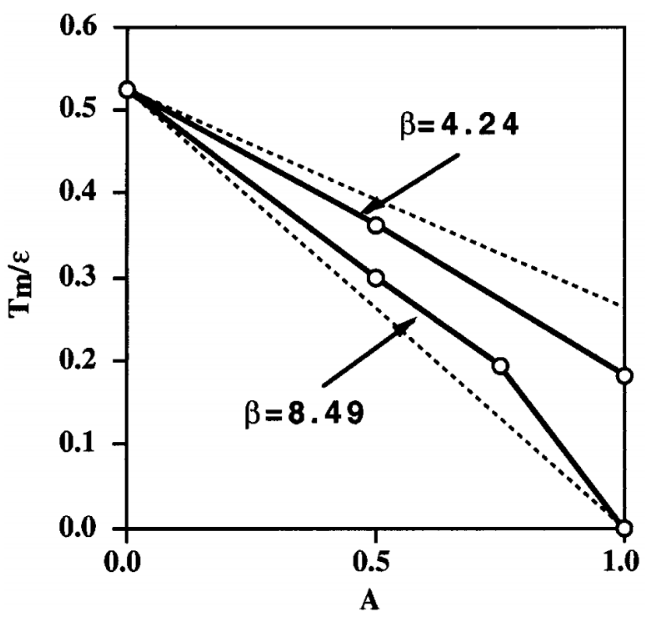
\includegraphics[width=0.50\textwidth]{temp_baskes}
\caption{Температура плавления в зависимости от $A$ и $\beta$ из статьи Baskes, “Many-Body Effects in fcc Metals”.}
\end{figure}
\FloatBarrier

Для проверки этого была получена стабильная решетка температуры >0.01 при $A=1.5 \ \beta=6$. Затем в течении 10 единиц времени она приводилась к необходимой температуре strong-coupling термостатом, после чего симулировалась до 30 единиц времени в NVE конфигурации. Это было произведено для температур 0.010 - 0.022 с шагом $10^{-3}$. Начиная с 0.019 в решетке появлялся центр плавления, после чего система быстро нагревалась, а ее функция радиального распределения принимала характерный вид для жидкости. Так же, был построен график критерия Линденманна, который дает такую же температуру плавления.

\begin{figure}[h]
\centering
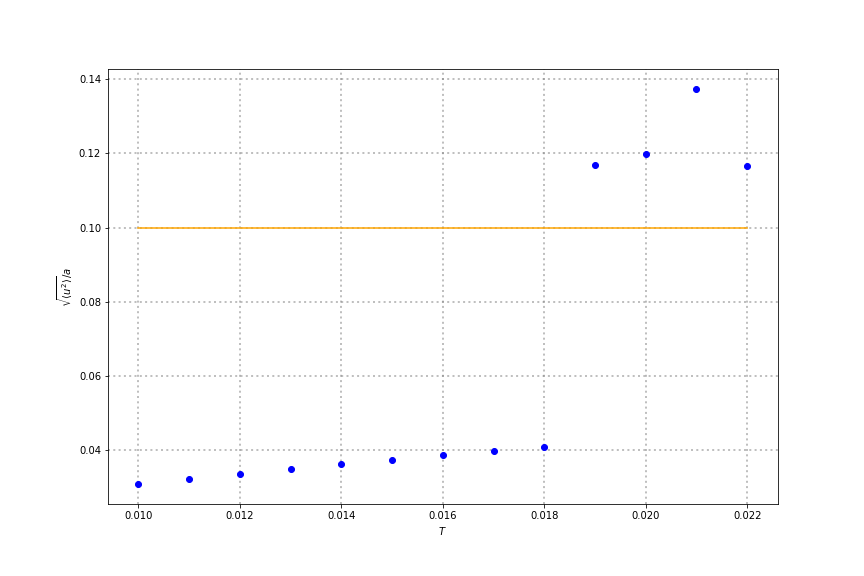
\includegraphics[width=1.0\textwidth]{lind}
\caption{Критерий Линденманна $N=512, A=1.5, \beta=6, \rho=0.512$}
\end{figure}
\FloatBarrier

Таким образом, EAM-LJ потенциал не позволяет получить стабильную dc-решетку при температурах, существенно отличных от 0.

\begin{figure}[h]
\centering
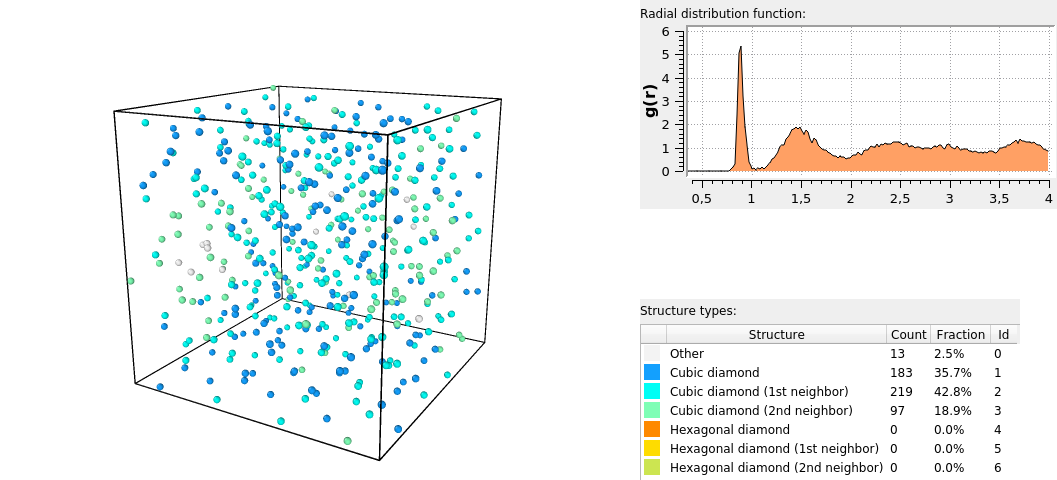
\includegraphics[width=0.8\textwidth]{temp_all}
\caption{dc(?)-решетка $N=512, A=10, \beta=7, \rho=1, T=0.65$}
\end{figure}
\FloatBarrier

Интересно рассмотреть dc-решетки при больших A на больших температурах. Можно увидеть, что вещество сохраняет структуру, не смотря на то, что RDF напоминает скорее жидкость, а колебания атомов вокруг положения равновесия превышают 10\% от растояния до ближайшего атома. Однако, разрушения решетки не происходит до некоторой температуры, в данном случае $T_m=0.78$.

\begin{figure}[h]
\centering
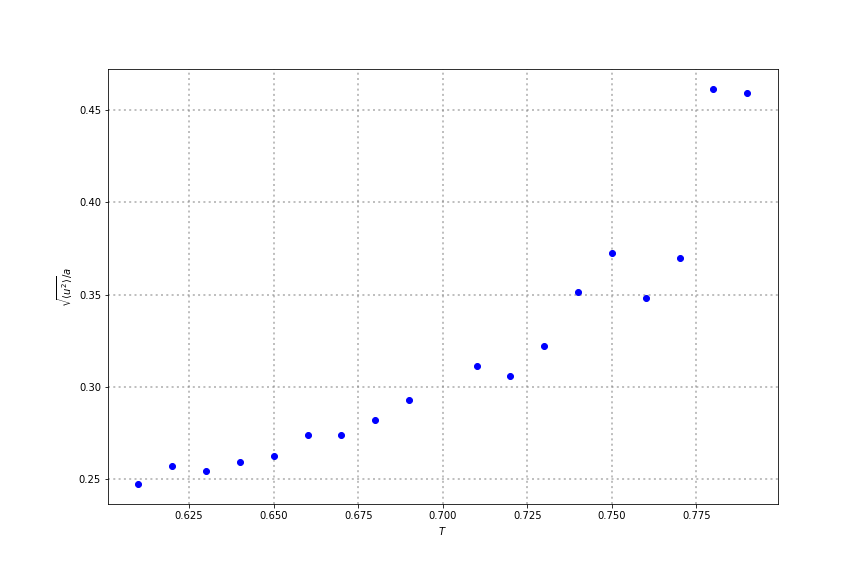
\includegraphics[width=0.8\textwidth]{lind_high}
\caption{Критерий Линденманна $N=512, A=10, \beta=7, \rho=1$}
\end{figure}
\FloatBarrier

Таким образом, когда взаимодействие по EAM потенциалу превыщает LJ взаимодействие, плавление может происходить по другому. В данном случае мы видим, что разрушение решетки происходит постепенно, начиная с потери 2х соседей. Для каких-либо выводов о характере этого являния требуются дальнейшие расчеты.

\subsection{Энергия формирования вакансии}
Так же можно посчитать энергию формирования вакансии в такой решетке. Получим релаксированную на 0 температуры решетку, посчитаем ее энергию, уберем атом и посчитаем энергию еще раз. Тогда энергия формирования вакансии будет определяться, как 
\begin{equation}
E_{v}^{f}=E_{f}-\left[\left(N_{0}-1\right) / N_{0}\right] * E_{i}
\end{equation}

где $E_i$ - энергия в идеальной решетке, $E_f$ - энергия системы после создания вакансии, $N_0$ - количество атомов до создания вакансии.

В нашем случае $E_i = -2442 \ E_f = -2435 \ N_0 = 512$. Тогда энергия формирования вакансии:
$E_v^f = 2$. Мне не удалось найти исследований для энергий вакансий в dc-решетках для такого потенциала, однако энергия формирования вакансии для никеля в EAM в [6] (для fcc-решетки, однако это оценка) имеет схожее значение (2,27 после пересчета в reduced units), так что можно предположить корректность полученных данных.

\section{Выводы}
В ходе выполнения проекта был реализован EAM-LJ потенциал и продемонстрированна корректность его работы. Были воспроизведены аналитические результаты работы [2] о возможности формирования решеток в этом потенциале. Так же были получены такие свойства dc-решетки, как температура плавления и энергия формирования вакансии, сходящиеся с представленными в статьях [2] и [6]. Помимо этого был получен эффект повышения температуры плавления для сильных потенциалов.


\newpage
\section{Литература}
\hspace{1.5em}[1] - M. S. Daw and M. I. Baskes, Phys. Rev. B 29, 6443 (1984).

[2] - M. I. Baskes, Phys. Rev. Lett. 83, 2592 (1999).

[3] - Honeycutt and Andersen, J. Phys. Chem. 91, 4950 (1987).

[4] - Maras, Emile, et al. "Global transition path search for dislocation formation in Ge on Si (001)." Computer Physics Communications 205 (2016): 13-21.

[5] - Stukowski, Alexander. "Visualization and analysis of atomistic simulation data with OVITO–the Open Visualization Tool." Modelling and Simulation in Materials Science and Engineering 18.1 (2009): 015012.

[6] - M. I. Baskes, Mater. Chem. Phys. 50, 152 (1997).
\end{document}